\documentclass[a4paper, 12pt]{article}
\usepackage{graphicx}
\usepackage[utf8]{inputenc}
\usepackage[T1]{fontenc}
\usepackage{lmodern}
\usepackage[danish]{babel}
\usepackage{amsmath}

\title{{\Huge Calculus}\\ En meget hurtig opsummering}
\date{\today}
\author{Jonas Camillus Jeppesen\thanks{jojep07@student.sdu.dk} \\
		Allan Grønhøj Hansen\thanks{alhan08@student.sdu.dk}}

\begin{document}
\maketitle
\newpage

\section{uge 1}
\begin{enumerate}
	\item Minimalt eksempel
	\item Overall skriftstørrelse
	\item Non-ascii
	\item Section og subsection
	\item Maketitle
	\item Indholdsfortegnelse
	\item Bable
	\item ref og label 
	\item begin end equation
\end{enumerate}

\section{uge 2}
\begin{enumerate}
	\item Lister (sublist)
	\item Align
	\item Matricer
	\item Spalter
	\item Tabeller
	\item Figurer
	\item include input
	\item bibliografi
\end{enumerate}
\newpage

\section{Introduktion}
Calculus er det matematiske studium af ændringer, på samme måde som geometri er det matematiske studium af former. 

\section{Differentiation}
Differentiation er et af de to store emner inden for calculus. Det handler om hvordan funktioner ændrer sig når deres input ændres. Et mål for dette er den \emph{aflede} af en funktion. 

\subsection{Definition af den aflede}
Hældningen af en sekantlinie til en funktion $f(x)$ i punktet $x_0$ er givet ved:
\begin{equation} \label{eq:diffquot}
s = \frac{f(x_0+h) - f(x_0)}{h}
\end{equation}
Denne brøk kaldes \emph{differenskvotienten}. Den aflede af en funktion i samme punkt er grænseværdien af ligning (\ref{eq:diffquot}) når $h\to0$:
\begin{equation} \label{eq:diffcoef}
m = \lim_{h\to0}\frac{f(x_0+h) - f(x_0)}{h}
\end{equation}
Denne grænse kaldes \emph{diffenskoefficienten}.  Figur \ref{fig:secanttangent} viser en funktion med en tangentlinie og to sekantlinier. Det ses, at når $h$ gøres mindre går hældningen af sekantlinierne mod hældningen af tangentlinien.
\begin{figure}[b]
	\centering
	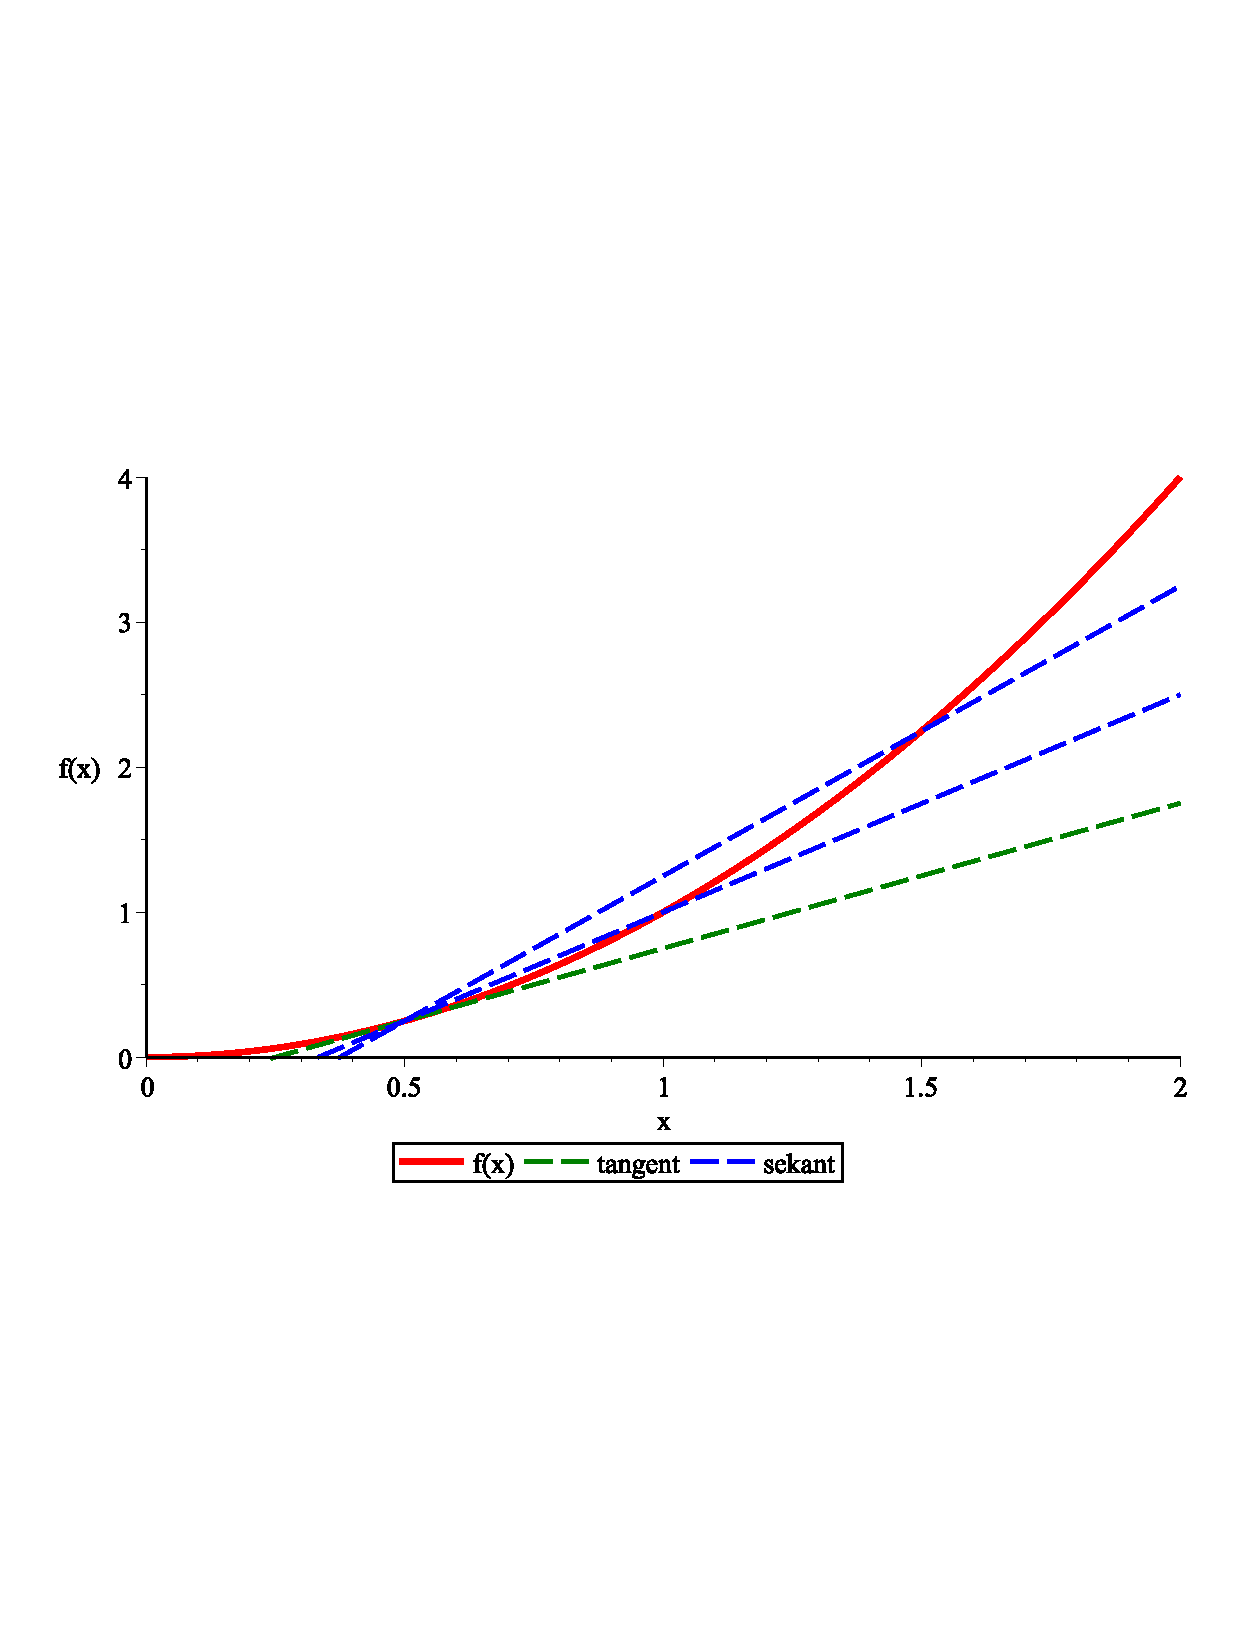
\includegraphics[width=0.8\textwidth, clip, trim=0 7.8cm 0 6cm]{secant}
	\caption{Afbildning af $f(x)=x^2$ med en tangent i punktet $x=0.5$ (grøn) og to sekantlinier (blå) med $h=0.5, 1.0$.}
	\label{fig:secanttangent}
\end{figure}

\subsection{Den aflede som funktion}
Hvis $f(x)$ har en aflede i alle punkter $a$ findes der en funktion som sender alle punkter $a$ over i den afledte af $f(x)$ i punktet $a$. Denne funktion kaldes \emph{den aflede funktion} af $f(x)$ og skrives som $\frac{df}{dx}$ i Leibnizs notation ($f'(x)$ i Lagranges notation).

Den aflede funktion kan bestemmes ud fra ligning (\ref{eq:diffcoef}). Tag for eksempel den aflede funktion af en potensfunktion $f(x) = x^n$:
\begin{align}
m =& \lim_{h\to0}\frac{f(x+h) - x^n}{h}
 =& \lim_{h\to0}\frac{(x+h)^n - x^n}{h}
\end{align}






\end{document}